\chapter{Semantics embedding}


\section{Traditional semantic representation}

\begin{description}
    \item[Lemma/citation form] \marginnote{Lemma}
        Syntactic form of a word.

        \begin{example}
            The word \texttt{pipe}.
        \end{example}

    \item[Word sense] \marginnote{Word sense}
        Meaning component of a word.

        \begin{description}
            \item[Polysemous lemma] Lemma with multiple senses. 
            \begin{example}
                Possible senses of the word \texttt{pipe} are: the music instrument, the conduit to transport material, \dots.
            \end{example}
        \end{description}

    \item[Supersense] \marginnote{Supersense}
        Semantic category for senses.

    \item[Word sense disambiguation (WSD)] \marginnote{Word sense disambiguation (WSD)}
        Task of determining the correct sense of a word.
\end{description}


\subsection{Sense relations}

\begin{description}
    \item[Synonym] \marginnote{Synonym}
        Relation of (near) identity between two senses of two different words (i.e., same propositional meaning).

        \begin{remark}[Principle of contrast]
            A different linguistic form is probably due to some, maybe subtle, difference in meaning.
        \end{remark}

    \item[Antonym] \marginnote{Antonym}
        Relation of opposition, with respect to one feature of meaning, between two senses. More specifically, antonyms can be:
        \begin{itemize}
            \item An opposition between two ends of a scale (e.g., \texttt{long}/\texttt{short}).
            \item A reversive (e.g., \texttt{up}/\texttt{down}).
        \end{itemize}

    \item[Subordination] \marginnote{Subordination}
        Specificity (i.e., is-a) relation between two senses.

        \begin{example}
            \texttt{car} is a subordinate of \texttt{vehicle}.
        \end{example}

    \item[Superordination] \marginnote{Superordination}
        Generalization relation between two senses.

        \begin{example}
            \texttt{furniture} is a superordinate of \texttt{lamp}.
        \end{example}

    \item[Meronym] \marginnote{Meronym}
        Part-of relation between two senses.
\end{description}

\begin{remark}
    Relations among word senses can be seen as a graph.
\end{remark}


\subsection{Common ontologies}

\begin{description}
    \item[WordNet] \marginnote{WordNet}
        Database of semantic relations of English words.

    \item[BabelNet] \marginnote{BabelNet}
        Multilingual database of semantic relations.
\end{description}


\subsection{Word relations}

\begin{description}
    \item[Word similarity] \marginnote{Word similarity}
        Measure the meaning similarity of words (i.e., relation between words and not senses).

        \begin{remark}
            Working with words is easier than senses.
        \end{remark}

        \begin{example}
            Cat and dog are not synonyms but have similar meaning (i.e., pets).
        \end{example}

    \item[Word relatedness] \marginnote{Word relatedness}
        Measure the context relation of words.

        \begin{example}
            \texttt{car}/\texttt{bike} are similar while \texttt{car}/\texttt{fuel} are related but not similar.
        \end{example}

        \begin{description}
            \item[Semantic field] \marginnote{Semantic field}
                Words that cover a particular domain and have structured relations with each other.

                \begin{example}
                    In the context of a hospital, \texttt{surgeon}, \texttt{scalpel}, \texttt{nurse}, \texttt{anesthetic}, and \texttt{hospital} belong to the same semantic field.
                \end{example}

                \begin{description}
                    \item[Topic model] \marginnote{Topic model}
                        Unsupervised method to cluster the topics in a document based on how a word is used in its context.
                \end{description}

            \item[Semantic frames] \marginnote{Semantic frames}
                Words that describe the perspective or participants of a particular event.

                \begin{example}
                    In a commercial transaction, a \texttt{buyer} trades \texttt{money} with a \texttt{seller} in return of some \texttt{good or service}.
                \end{example}

                \begin{description}
                    \item[Semantic role labeling (SRL)] \marginnote{Semantic role labeling (SRL)}
                        Task of determining the frames and their semantic role.
                \end{description}
        \end{description}
\end{description}


\section{Vector semantics}

\begin{description}
    \item[Connotation] \marginnote{Connotation}
        Affective meaning of a word.

        \begin{remark}
            As described in \Cref{sec:affective_meaning}, emotions can be represented in a vector space. Therefore, word meanings can also be represented as vectors.
        \end{remark}

    % \item[Vector semantics] \marginnote{Vector semantics}
    %     Define a word by its environment or distribution in language use.
    
    \item[Vector semantics intuitions]
        Vector semantics lay on two intuitions:
        \begin{descriptionlist}
            \item[Distributionalism intuition] \marginnote{Distributionalism intuition}
                The meaning of a word is defined by its environment or distribution (i.e., neighboring words). Words with a similar distribution are likely to have the same meaning.

            \item[Vector intuition] \marginnote{Vector intuition}
                Define the meaning of a word as a point in an $N$-dimensional space.
        \end{descriptionlist}

    \item[Embedding] \marginnote{Embedding}
        Vector representation of a word where words with a similar meaning are nearby in the vector space.

        Two common embedding models are:
        \begin{descriptionlist}
            \item[TF-IDF] \marginnote{TF-IDF}
                Sparse embedding based on the counts of nearby words.

            \item[Word2vec] \marginnote{Word2vec}
                Dense embedding learned by training a classifier to distinguish nearby and far-away words.
        \end{descriptionlist}
\end{description}


\subsection{Sparse embeddings}

\begin{description}
    \item[Co-occurrence matrix] \marginnote{Co-occurrence matrix}
        Matrix representing the frequency that words occur with the others.

        Different design choices can be considered:
        \begin{itemize}
            \item Matrix design.
            \item Reweighing.
            \item Dimensionality reduction.
            \item Vector comparison metric.
        \end{itemize}

    \item[Matrix design] 
        Shape and content of the co-occurrence matrix.

        \begin{description}
            \item[Term-document matrix] \marginnote{Term-document matrix}
                Given a vocabulary $V$ and a set of documents $D$, a term-document matrix has shape $|V| \times |D|$ and counts the occurrences of each word in each document.

                \begin{remark}
                    This representation allows to encode both documents (i.e., by considering the matrix column-wise) and words (i.e., by considering the matrix row-wise).
                \end{remark}

                \begin{example}
                    An excerpt of a possible term-document matrix for Shakespeare is:
                    \begin{table}[H]
                        \centering
                        \footnotesize
                        \begin{tabular}{ccccc}
                            \toprule
                            & \textit{As You Like It} & \textit{Twelfth Night} & \textit{Julius Caesar} & \textit{Henry V} \\
                            \midrule
                            \texttt{battle} & 1 & 0 & 7 & 13 \\
                            \texttt{good} & 114 & 80 & 62 & 89 \\
                            \texttt{fool} & 36 & 58 & 1 & 4 \\
                            \texttt{wit} & 20 & 15 & 2 & 3 \\
                            \bottomrule
                        \end{tabular}
                    \end{table}
                    The representation for the document \textit{As You Like It} is $[1, 114, 36, 20]$, while the representation of the word \texttt{battle} is $[1, 0, 7, 13]$.
                \end{example}

            \item[Word-word matrix] \marginnote{Word-word matrix}
                Given a vocabulary $V$, a word-word matrix has shape $|V| \times |V|$. Rows represent target words and columns are context words.
                Given a training corpus, the word at each row is represented by counting its co-occurrences with the others within a context of $N$ words.

                \begin{remark}
                    A larger context window captures more semantic information. A smaller window captures more syntactic information.
                \end{remark}

                \begin{example}
                    A possible word-word matrix is:
                    \begin{table}[H]
                        \centering
                        \footnotesize
                        \begin{tabular}{ccccccccc}
                            \toprule
                            & \texttt{aardvark} & \dots & \texttt{computer} & \texttt{data} & \texttt{result} & \texttt{pie} & \texttt{sugar} & \dots \\
                            \midrule
                            \texttt{cherry} & 0 & \dots & 2 & 8 & 9 & 442 & 25 & \dots \\
                            \texttt{strawberry} & 0 & \dots & 0 & 0 & 1 & 60 & 19 & \dots \\
                            \texttt{digital} & 0 & \dots & 1670 & 1683 & 85 & 5 & 4 & \dots \\
                            \texttt{information} & 0 & \dots & 3325 & 3982 & 378 & 5 & 13 & \dots \\
                            \bottomrule
                        \end{tabular}
                    \end{table}
                \end{example}
        \end{description}

    \item[Reweighing] 
        Rescale the vectors to emphasize important features and down-weigh irrelevant words.

        \begin{remark}[Frequency paradox]
            Raw frequencies are not an ideal representation for words as they are skewed and not discriminative. Moreover, overly frequent words (e.g., stop words) do not provide context information.
        \end{remark}

        \begin{description}
            \item[Term frequency-inverse document frequency (TF-IDF)] \marginnote{Term frequency-inverse document frequency (TF-IDF)}
                Based on term-document occurrences. Given a word $t$ and a document $d$, it is computed as:
                \[ \texttt{tf-idf}(t, d) = \texttt{tf}(t, d) \cdot \texttt{idf}(t) \]
                where:
                \begin{descriptionlist}
                    \item[Term frequency (\texttt{tf})] 
                        Log-transformed frequency count of a word $t$ in a document $d$:
                        \[ 
                            \texttt{tf}(t, d) = \begin{cases}
                                1 + \log_{10}\left( \texttt{count}(t, d) \right) & \text{if $\texttt{count}(t, d) > 0$} \\
                                0 & \text{otherwise}
                            \end{cases} 
                        \]

                    \item[Inverse document frequency (\texttt{idf})]
                        Inverse occurrence count of a word $t$ across all documents:
                        \[ \texttt{idf}(t) = \log_{10}\left( \frac{N}{\texttt{df}_t} \right) \]
                        where $\texttt{df}_t$ is the number of documents in which the term $t$ occurs.

                        \begin{remark}
                            Words that occur in a few documents have a high \texttt{idf}. Therefore, stop words, which appear often, have a low \texttt{idf}.
                        \end{remark}
                \end{descriptionlist}

                \begin{example}
                    Consider the term-document matrix with \texttt{tf} in parentheses:
                    \begin{table}[H]
                        \centering
                        \footnotesize
                        \begin{tabular}{ccccc}
                            \toprule
                            & \textit{As You Like It} & \textit{Twelfth Night} & \textit{Julius Caesar} & \textit{Henry V} \\
                            \midrule
                            \texttt{battle} & 1 ($1$) & 0 ($0$) & 7 ($1.845$) & 13 ($2.114$) \\
                            \texttt{good} & 114 ($3.057$) & 80 ($2.903$) & 62 ($2.792$) & 89 ($2.949$) \\
                            \texttt{fool} & 36 ($2.553$) & 58 ($2.763$) & 1 ($1$) & 4 ($1.602$) \\
                            \texttt{wit} & 20 ($2.301$) & 15 ($2.176$) & 2 ($1.301$) & 3 ($1.477$) \\
                            \bottomrule
                        \end{tabular}
                    \end{table}
                    Assume that the \texttt{df} and \texttt{idf} of the words are:
                    \begin{table}[H]
                        \centering
                        \footnotesize
                        \begin{tabular}{ccc}
                            \toprule
                            \textbf{Word} & \texttt{df} & \texttt{idf} \\
                            \midrule
                            \texttt{battle} & $21$ & $0.246$ \\
                            \texttt{good} & $37$ & $0$ \\
                            \texttt{fool} & $36$ & $0.012$ \\
                            \texttt{wit} & $34$ & $0.037$ \\
                            \bottomrule
                        \end{tabular}
                    \end{table}
                    The resulting TF-IDF weighted matrix is:
                    \begin{table}[H]
                        \centering
                        \footnotesize
                        \begin{tabular}{ccccc}
                            \toprule
                            & \textit{As You Like It} & \textit{Twelfth Night} & \textit{Julius Caesar} & \textit{Henry V} \\
                            \midrule
                            \texttt{battle} & $0.246$ & 0 & $0.454$ & $0.520$ \\
                            \texttt{good} & 0 & 0 & 0 & 0 \\
                            \texttt{fool} & $0.030$ & $0.033$ & $0.001$ & $0.002$ \\
                            \texttt{wit} & $0.085$ & $0.081$ & $0.048$ & $0.054$ \\
                            \bottomrule
                        \end{tabular}
                    \end{table}
                \end{example}

            \item[Positive point-wise mutual information (PPMI)] \marginnote{Positive point-wise mutual information (PPMI)}
                Based on term-term occurrences. Given a word $w$ and a context word $c$, it determines whether they are correlated or occur by chance as follows:
                \[ \texttt{PPMI}(w, c) = \max\left\{ \texttt{PMI}(w, c), 0 \right\} \]
                where:
                \begin{descriptionlist}
                    \item[Point-wise mutual information (\texttt{PMI})]
                    \[ \texttt{PMI}(w, c) = \log_2\left( \frac{\prob{w, c}}{\prob{w}\prob{c}} \right) \in (-\infty, +\infty) \]
                    where:
                    \begin{itemize}
                        \item The numerator is the probability that $w$ and $c$ co-occur by correlation.
                        \item The denominator is the probability that $w$ and $c$ co-occur by chance.
                    \end{itemize} 

                    \begin{remark}
                        $\texttt{PMI} > 1$ indicates correlated co-occurrence. Otherwise, it is by chance.
                    \end{remark}
                \end{descriptionlist}

                \begin{remark}[Weighting \texttt{PPMI}]
                    \texttt{PMI} is biased towards infrequent events and returns very high values for them. This can be solved by either:
                    \begin{itemize}
                        \item Using add-$k$ smoothing (typically, $k \in [0.1, 3]$).
                        \item Slightly increasing the probability of rare context words such that $\mathcal{P}_\alpha(c) = \frac{\texttt{count}(c)^\alpha}{\sum_{c'}\texttt{count}(c')^\alpha}$ (typically, $\alpha=0.75$).
                    \end{itemize}
                \end{remark}

                \begin{example}
                    Consider the term-term matrix:
                    \begin{table}[H]
                        \centering
                        \footnotesize
                        \begin{tabular}{cccccc|c}
                            \toprule
                            & \texttt{computer} & \texttt{data} & \texttt{result} & \texttt{pie} & \texttt{sugar} & $\texttt{count}(w)$ \\
                            \midrule
                            \texttt{cherry} & $2$ & $8$ & $9$ & $442$ & $25$ & $486$ \\
                            \texttt{strawberry} & $0$ & $0$ & $1$ & $60$ & $19$ & $80$ \\
                            \texttt{digital} & $1670$ & $1683$ & $85$ & $5$ & $4$ & $3447$ \\
                            \texttt{information} & $3325$ & $3982$ & $378$ & $5$ & $13$ & $7703$ \\
                            \midrule
                            $\texttt{count}(c)$ & $4977$ & $5673$ & $473$ & $512$ & $61$ & $11716$ \\
                            \bottomrule
                        \end{tabular}
                    \end{table}
                    The PPMI between \texttt{information} and \texttt{data} con be computed as:
                    \[
                        \begin{split}
                            \prob{\texttt{information}, \texttt{data}} &= \frac{3982}{11716} = 0.3399 \\
                            \prob{\texttt{information}} &= \frac{7703}{11716} = 0.6575 \\
                            \prob{\texttt{data}} &= \frac{5673}{11716} = 0.4872 \\
                            \texttt{PPMI}(\texttt{information}, \texttt{data}) &= \max\left\{ \log_2\left( \frac{0.3399}{0.6575 \cdot 0.4872} \right), 0 \right\} = 0.0944
                        \end{split}
                    \]
                \end{example}
        \end{description}

        \begin{remark}
            Reweighing loses information about the magnitude of the counts.
        \end{remark}

    \item[Dimensionality reduction] 
        Reduce the dimensionality of the embeddings.

    \item[Vector comparison] 
        Metric to determine the distance of two embeddings.

        \begin{description}
            \item[Dot product] $\vec{w} \cdot \vec{v} = \sum_{i=1}^{n} w_i v_i$.
            \item[Length] Compare the length $|\vec{v}| = \sqrt{\sum_{i=1}^{n} v_i^2}$ of the vectors.
            \item[Cosine similarity] $\frac{\vec{w} \cdot \vec{v}}{|\vec{w}| \, |\vec{v}|}$.
        \end{description}
\end{description}


\subsection{Dense non-contextual embeddings}

\begin{remark}
    Dense embeddings are usually:
    \begin{itemize}
        \item Easier to process with machine learning algorithms.
        \item Able to generalize better than simply counting.
        \item Handle synonyms better.
    \end{itemize}
\end{remark}

\begin{description}
    \item[Neural language modeling] \marginnote{Neural language modeling}
        Use a neural network to predict the next word $w_{n+1}$ given an input sequence $w_{1..n}$. The general flow is the following:
        \begin{enumerate}
            \item Encode the input words into one-hot vectors ($\mathbb{R}^{|V| \times n}$). 
            \item Project the input vectors with an embedding matrix $\matr{E} \in \mathbb{R}^{d \times |V|}$ that encodes them into $d$-dimensional vectors.
            \item Pass the embedding into the hidden layers.
            \item The final layer is a probability distribution over the vocabulary ($\mathbb{R}^{|V| \times 1}$).
        \end{enumerate}

        \begin{figure}[H]
            \centering
            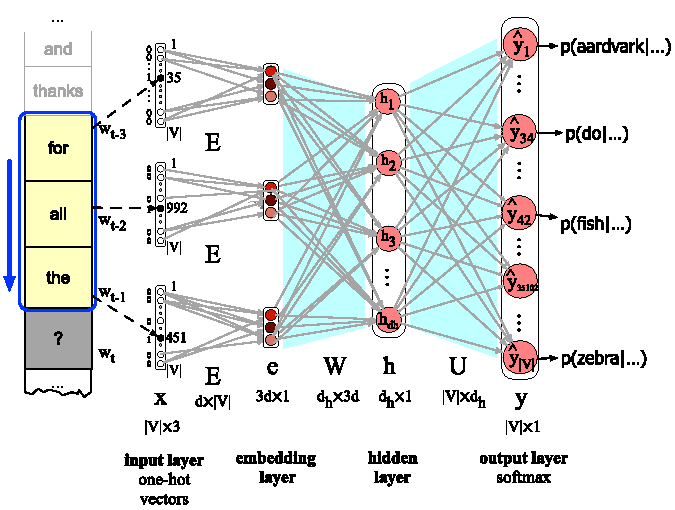
\includegraphics[width=0.6\linewidth]{./img/_neural_language_model_example.pdf}
            \caption{Example of neural language model with a context of $3$ tokens}
        \end{figure}

        \begin{remark}
            The embedding matrix $\matr{E}$ can be used independently to embed words. In fact, by construction, the $i$-th column of $\matr{E}$ represents the embedding of the $i$-th token of the vocabulary.
        \end{remark}

        \begin{description}
            \item[Training] 
                Given a text corpus, training is done sequentially in a self-supervised manner by sliding a context window over the sequence. At each iteration, the next word is predicted and cross-entropy is used as loss.

                \begin{remark}
                    The initial embedding matrix is usually initialized using statistical methods and not randomly.
                \end{remark}
        \end{description}

    \item[Word2vec] \marginnote{Word2vec}
        Word embedding framework that encodes a target word based on the context words near it.

        Two training variants are available in Word2vec:
        \begin{descriptionlist}
            \item[Continuous bag-of-words (CBOW)]
                Given the context words, predict the target word.

            \item[Skip-gram]
                Given the target word, predict the (position independent) context words.
        \end{descriptionlist}

        \begin{figure}[H]
            \centering
            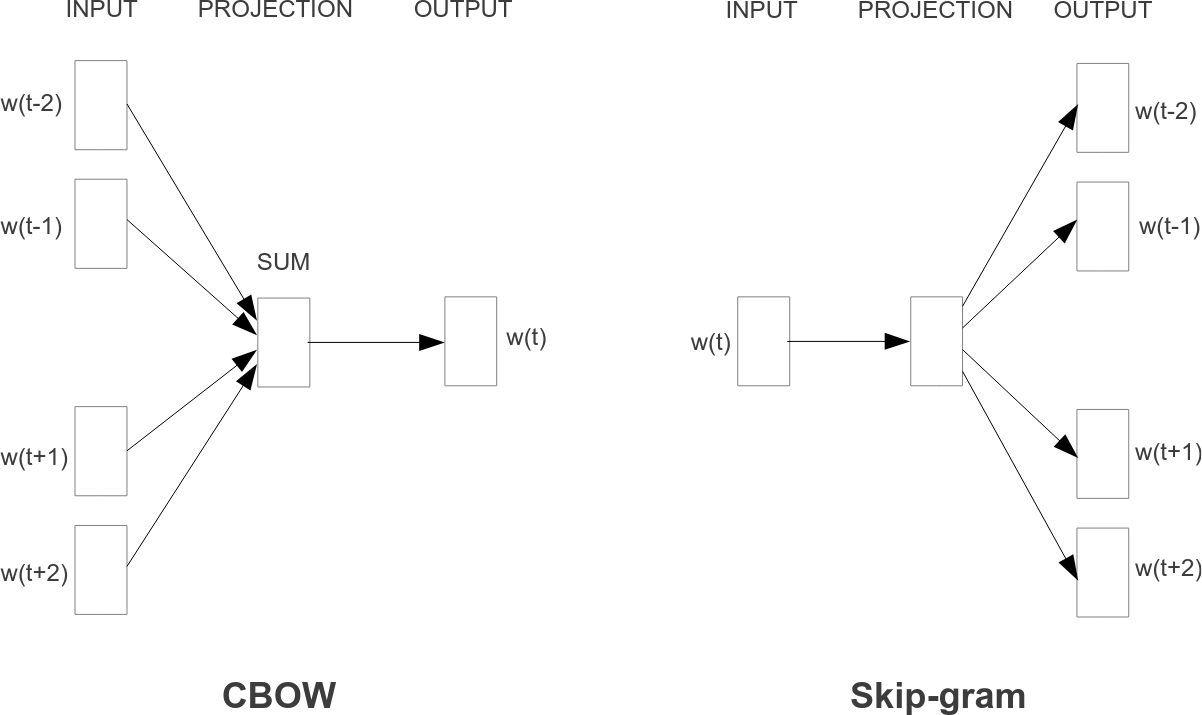
\includegraphics[width=0.5\linewidth]{./img/word2vec_alternatives.png}
        \end{figure}

        \begin{description}
            \item[Skip-gram model] \marginnote{Skip-gram model}
                Given a context word $c$ and a target word $w$, a classifier is trained to determine whether $c$ appears in the context of $w$. After training, the weights of the classifier are used as the skip-gram model to embed words.

                \begin{remark}
                    In practice, for an easier optimization, the skip-gram model learns two sets of embeddings $\matr{W} \in \mathbb{R}^{|V| \times d}$ and $\matr{C} \in \mathbb{R}^{|V| \times d}$ for the target and context words, respectively. Therefore, it has two sets of parameters $\matr{\theta} = \langle\matr{W}, \matr{C}\rangle$. At the end, they can either be averaged, concatenated, or one can be dropped.
                \end{remark}

                \begin{description}
                    \item[Training (softmax)]
                        Given the target word $w$ and context word $c$, and their embeddings $\vec{w}$ and $\vec{c}$, the skip-gram model computes their similarity as the dot product. The probability that $c$ is in the context of $w$ is then computed though a softmax as:
                        \[ 
                            \prob{c | w; \matr{\theta}} = \frac{\exp(\vec{c} \cdot \vec{w})}{\sum_{v \in V} \exp(\vec{v} \cdot \vec{w})}
                        \]

                        Given a training sequence $w_1, \dots, w_T$ and a context window of size $m$, training is done by iterating over each possible target word $w_t$ and considering the conditional probabilities of its neighbors. Then, the loss is defined as the average negative log-likelihood defined as follows:
                        \[
                            \begin{split}
                                \mathcal{L}(\matr{\theta}) = -\frac{1}{T} \sum_{t=1}^{T} \sum\limits_{\substack{-m \leq j \leq m\\j \neq 0}} \log\left( \prob{w_{t+j} | w_t; \matr{\theta}} \right)
                            \end{split}
                        \]

                        \begin{remark}
                            Due to the normalization factor over the whole vocabulary, using softmax for training is expensive.
                        \end{remark}

                    \item[Training (negative sampling)] \marginnote{Skip-gram with negative sampling (SGNS)}
                        Use a binary logistic regressor as classifier. The two classes are:
                        \begin{itemize}
                            \item Context words within the context window (positive label).
                            \item Words randomly sampled (negative label).
                        \end{itemize} 
                        The probabilities can be computed as:
                        \[ 
                            \prob{\texttt{+} | w, c; \matr{\theta}} = \sigma(\vec{c} \cdot \vec{w}) 
                            \qquad
                            \prob{\texttt{-} | w, c; \matr{\theta}} = 1 - \prob{\texttt{+} | w, c; \matr{\theta}}
                        \]

                        It is assumed context-independent words, therefore, if the context is a sequence, the probability is computed as follows:
                        \[ \prob{\texttt{+} | w, c_{1..L}; \matr{\theta}} = \prod_{i=1}^{L} \sigma(\vec{c}_i \cdot \vec{w}) \]

                        At each iteration, the batch is composed of a single positive examples and $K$ negative examples randomly sampled according to their weighted unigram probability $\mathcal{P}_\alpha(w) = \frac{\texttt{count}(w)^\alpha}{\sum_{v \in V} \texttt{count}(v)^\alpha}$ ($\alpha$ it used to give rarer words a slightly higher probability).

                        Given a batch, the loss is defined as:
                        \[
                            \begin{split}
                                \mathcal{L}(\matr{\theta}) &= -\log\left( \prob{\texttt{+} | w, c^\text{pos}; \matr{\theta}} \prod_{i=1}^{K} \prob{\texttt{-} | w, c^\text{neg}_{i}; \matr{\theta}} \right) \\
                                &= - \left( \log\left( \sigma(\vec{c}^\text{pos} \cdot \vec{w}) \right) + \sum_{i=1}^{K} \log\left( \sigma(-\vec{c}^\text{neg}_{i} \cdot \vec{w}) \right) \right)
                            \end{split}
                        \]
                \end{description}
        \end{description}


    \item[fastText] \marginnote{fastText}
        Extension of Word2vec based on subwords to deal with out-of-vocabulary words.

        A word is represented both as itself and a bag of $n$-grams. Both whole words and $n$-grams have an embedding. The overall embedding of a word is represented through the sum of its constituent $n$-grams.

        \begin{example}
            With $n=3$, the word \texttt{where} is represented both as \texttt{<where>} and \texttt{<wh, whe, her, ere, re>} (\texttt{<} and \texttt{>} are boundary characters).
        \end{example}

    \item[GloVe] \marginnote{GloVe}
        Based on the term-term co-occurrence (within a window) probability matrix that indicates for each word its probability of co-occurring with the other words.

        Similarly to Word2vec, the objective is to learn two sets of embeddings $\matr{\theta} = \langle\matr{W}, \matr{C}\rangle$ such that their similarity is close to their log-probability of co-occurring. Given the term-term matrix $\matr{X}$, the loss for a target word $w$ and a context word $c$ is defined as:
        \[ \mathcal{L}(\matr{\theta}) = \left( \vec{c} \cdot \vec{w} - \log( \matr{X}[c, w] ) \right)^2 \]

        \begin{remark}
            Empirically, for GloVe it has been observed that the final embedding matrix obtain as $\matr{W} + \matr{C}$ works better.
        \end{remark}

        \begin{example}
            A possible term-term co-occurrence probability for the words \texttt{ice} and \texttt{steam} is the following:
            \begin{table}[H]
                \centering
                \footnotesize
                \begin{tabular}{ccccc}
                    \toprule
                    & $k=\texttt{solid}$ & $k=\texttt{gas}$ & $k=\texttt{water}$ & $k=\texttt{fashion}$ \\
                    \midrule
                    $\prob{k | \texttt{ice}}$ & $1.9 \times 10^{-4}$ & $6.6 \times 10^{-5}$ & $3.0 \times 10^{-3}$ & $1.7 \times 10^{-5}$ \\
                    $\prob{k | \texttt{steam}}$ & $2.2 \times 10^{-5}$ & $7.8 \times 10^{-4}$ & $2.2 \times 10^{-3}$ & $1.8 \times 10^{-5}$ \\
                    \bottomrule
                \end{tabular}
            \end{table}
            \texttt{ice} is more likely to co-occur with \texttt{solid} while \texttt{steam} is more likely to co-occur with \texttt{gas}. GloVe uses this information when determining the embeddings.
        \end{example}
\end{description}



\section{Embeddings properties}


\subsection{Embeddings similarity}

\begin{description}
    \item[Context size] \marginnote{Context size}
        The window size used to collect counts or determine context words can result in different embeddings.

        As a general rule, smaller windows tend to capture more syntactic features while a larger window encodes more topically related but not necessarily similar words.

    \item[Similarity orders] \marginnote{Similarity orders}
        Two words have:
        \begin{descriptionlist}
            \item[First-order co-occurrence] 
                If they are nearby each other.
            \item[Second-order co-occurrence] 
                If they have similar context words.
        \end{descriptionlist}

    \item[Relational similarity] \marginnote{Relational similarity}
        Dense embeddings are able to capture relational meanings.

        \begin{figure}[H]
            \centering
            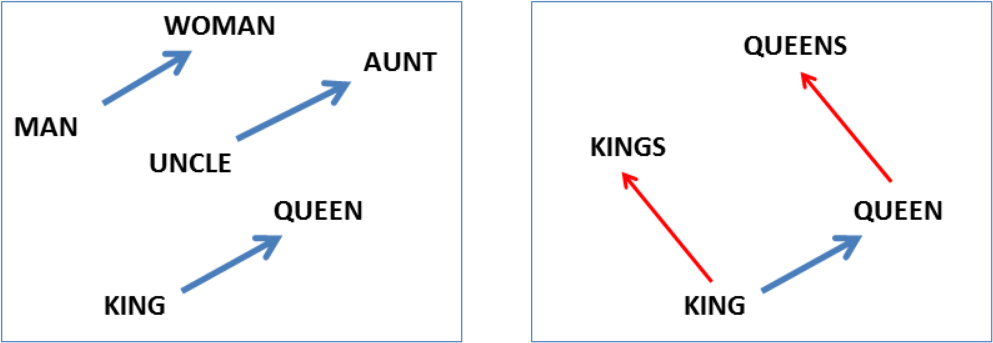
\includegraphics[width=0.45\linewidth]{./img/embedding_relations.png}
        \end{figure}

        \begin{description}
            \item[Parallelogram model] 
                Given the problem ``$a \text{ is to } b \text{ as } a^* \text{ is to } b^*$'' ($a : b :: a^* : b^*$), the parallelogram model solves it as:
                \[ b^* = \arg\min_x \texttt{distance}(x, b-a+a^*) \]

                \begin{example}
                    In Word2vec, the following operation between embeddings can be done:
                    \[ \texttt{Paris} - \texttt{France} + \texttt{Italy} \approx \texttt{Rome} \]
                \end{example}

                \begin{remark}
                    Even if it sometimes works, parallelogram model is not guaranteed to always produce the expected result.
                \end{remark}
        \end{description}
\end{description}


\subsection{Embeddings analysis}

\begin{description}
    \item[Word history] \marginnote{Word history}
        Trained on different corpora, dense embeddings can provide a semantic evolution of words by analyzing its neighboring embeddings.

        \begin{example}
            \phantom{}
            \begin{figure}[H]
                \centering
                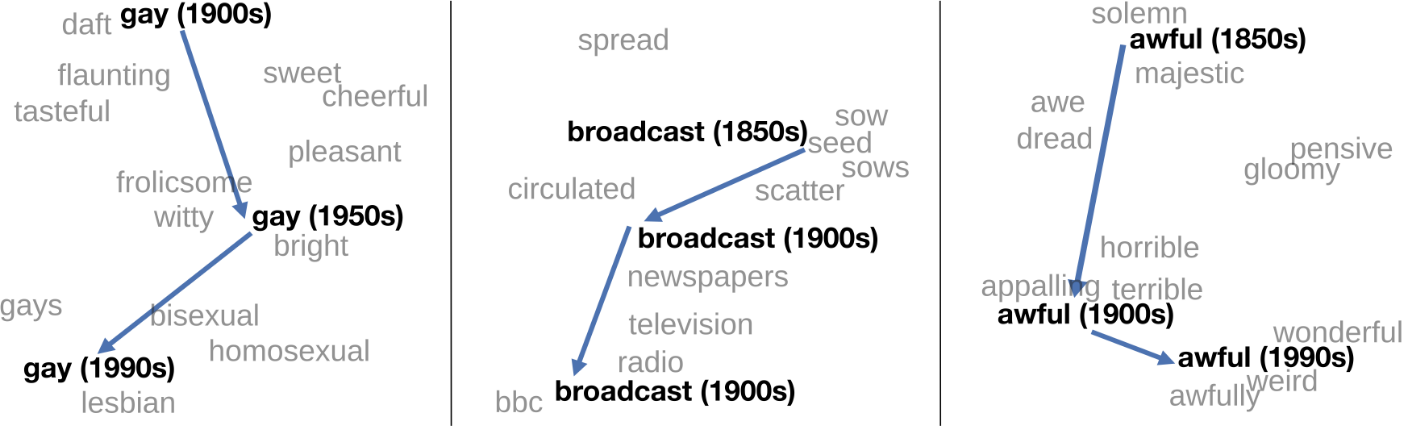
\includegraphics[width=0.7\linewidth]{./img/_embedding_history.png}
                \caption{
                    \parbox[t]{0.7\linewidth}{
                        Neighboring embeddings of the same words encoded using Word2vec trained on different corpora from different decades
                    }
                }
            \end{figure}
        \end{example}

        \begin{example}
            \phantom{}
            \begin{figure}[H]
                \centering
                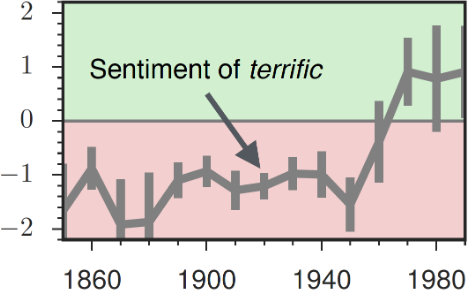
\includegraphics[width=0.25\linewidth]{./img/embedding_sentiment_history.png}
                \caption{
                    \parbox[t]{0.7\linewidth}{
                        Sentiment for the word \texttt{terrific} analyzed using the embeddings obtained by training on different corpora
                    }
                }
            \end{figure}
        \end{example}

    \item[Cultural bias] \marginnote{Cultural bias}
        Embeddings reflect implicit biases in the training corpus.

        \begin{description}
            \item[Implicit association test] 
                Determine how associated are concepts and attributes.

                \begin{example}
                    Using the parallelogram model to solve:
                    \[ \texttt{father} : \texttt{doctor} :: \texttt{mother} : x \]
                    finds as the closest words $x =$ \texttt{homemaker}, \texttt{nurse}, \texttt{receptionist}, \dots
                \end{example}

                \begin{example}
                    African-American and Chinese names are closer to unpleasant words compared to European-American names.
                \end{example}

                \begin{example}
                    Using the Google News dataset as training corpus, there is a correlation between the women bias of the jobs embeddings and the percentage of women over men in those jobs.

                    Woman bias for a word $w$ is computed as:
                    \[ d_\text{women}(w) - d_\text{men}(w) \]
                    where $d_\text{women}(w)$ is the average embedding distance between words representing women (e.g., \texttt{she}, \texttt{female}, \dots) and the word $w$. The same idea is applied to $d_\text{men}(w)$.

                    \begin{figure}[H]
                        \centering
                        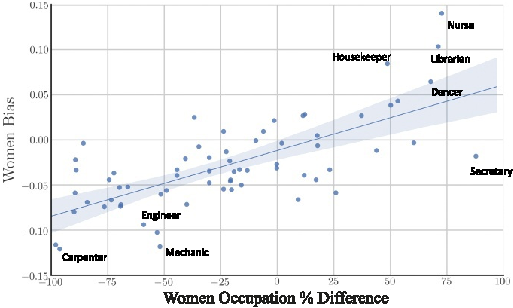
\includegraphics[width=0.6\linewidth]{./img/_embedding_women_occupation.pdf}
                        \caption{
                            \parbox[t]{0.7\linewidth}{
                                Relationship between the relative percentage of women in an occupation and the women bias.
                            }
                        }
                    \end{figure}

                    \begin{figure}[H]
                        \centering
                        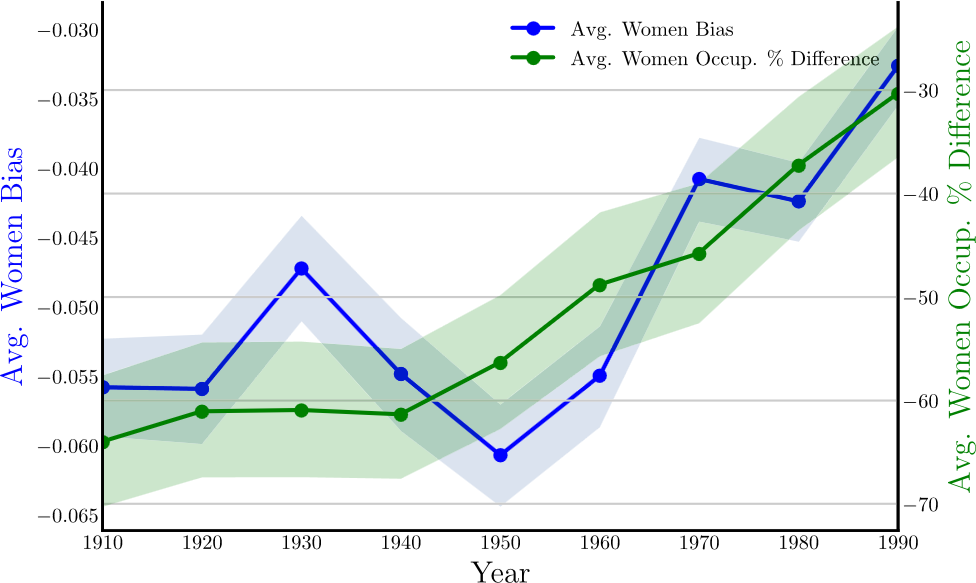
\includegraphics[width=0.6\linewidth]{./img/embedding_women_occupation_bias.png}
                        \caption{
                            \parbox[t]{0.7\linewidth}{
                                Average women bias vs average women occupation difference over time.
                            }
                        }
                    \end{figure}
                \end{example}
        \end{description}
\end{description}